\documentclass[11pt, letterpaper]{article}
\setlength{\parindent}{0in}
\setlength{\textheight}{8.7in}
\setlength{\textwidth}{6.8in}
\setlength{\oddsidemargin}{-0.3in}
\setlength{\evensidemargin}{0.0in}
\addtolength{\topmargin}{-1in}
\setlength{\parskip}{0.1in}

\usepackage{amsmath, amsfonts, amssymb, color}
\usepackage{bm}
\usepackage{booktabs}
\usepackage{enumerate}
\usepackage{graphicx}
\usepackage{pdfpages}
\newcommand*{\justifyheading}{\raggedleft}


\renewcommand{\baselinestretch}{1.0}

\newcommand{\bx}{{\bm x}}
\newcommand{\bX}{{\bm X}}
\newcommand{\by}{{\bm y}}
\newcommand{\bY}{{\bm Y}}
\newcommand{\bW}{{\bm W}}
\newcommand{\bG}{{\bm G}}
\newcommand{\bR}{{\bm R}}
\newcommand{\bZ}{{\bm Z}}
\newcommand{\bV}{{\bm V}}
\newcommand{\bL}{{\bm L}}
\newcommand{\bz}{{\bm z}}
\newcommand{\be}{{\bm e}}
\newcommand{\bgamma}{{\bm \gamma}}
\newcommand{\bbeta}{{\bm \beta}}
\newcommand{\balpha}{{\bm \alpha}}
\newcommand{\bSigma}{{\bm \Sigma}}
\newcommand{\bmu}{{\bm \mu}}
\newcommand{\btheta}{{\bm \theta}}
\newcommand{\bepsilon}{{\bm \epsilon}}
\newcommand{\bone}{{\bm 1}}
\newcommand{\bzero}{{\bm 0}}
\newcommand{\bC}{{\bm C}}
\newcommand{\bI}{{\bm I}}
\newcommand{\bA}{{\bm A}}
\newcommand{\bB}{{\bm B}}
\newcommand{\bQ}{{\bm Q}}
\newcommand{\bS}{{\bm S}}
\newcommand{\bD}{{\bm D}}
\newcommand{\cQ}{\mathcal{Q}}
\newcommand{\cU}{\mathcal{U}}
\newcommand{\cI}{\mathcal{I}}
\newcommand{\cL}{\mathcal{L}}

\newcommand{\beas}{\begin{eqnarray*}}
\newcommand{\eeas}{\end{eqnarray*}}

\newenvironment{equationarrayright}{
                          \begin{eqnarray*}
                          \begin{array}{rcll}
                         }{
                          \end{array}
                          \end{eqnarray*}
                         }
\newcommand{\bear}{\begin{equationarrayright}}
\newcommand{\eear}{\end{equationarrayright}}

\renewcommand\arraystretch{1.3}

\DeclareMathOperator*{\argmin}{arg\,min}

\title{STAT/BIOST 571: Homework 7}
\author{Philip Pham}
\date{\today}

\begin{document}

\maketitle

\section*{Problem 1: Relationship between fixed effects, random effects, GLS, and penalized regression; confounding; model misspecification (20 points)} 

{\em This is an extension of problem  3 from homework 1.  There are $n$ subjects, indexed by $i=1,\ldots,n$, each one of which is observed at
$m$ follow-up times, indexed by $j=1,\ldots,m$.  Let $Y_{ij}$ be the literacy score of subject $i$ at follow-up time $j$, at which time the subject's age is $x_{ij}$.  
The design is fixed, meaning that the $x_{ij}$ are all
deterministic and known in advance, and the true data-generating
mechanism can be written
\[
Y_{ij}=f(x_{i1})+\beta_L(x_{ij}-x_{i1})+\epsilon_{ij}
\]
with i.i.d. $\epsilon_{ij}\sim N(0,\sigma^2)$.  We are interested in estimating $\beta_L$,
without knowing the form of $f(x)$.
For this problem, fix $n=91$ and $m=3$, set 
the initial follow-up age for subject $i$ to be 
\[
x_{i1}=1+0.1*(i-1),
\]
have subsequent follow-ups evenly spaced at intervals of 
\[
\Delta x_i = \left(1 + \frac{10-x_{i1}}{10}\right)^2,
\]
and consider the fixed (but unknown) mean model implied by $\beta_L=1$ and  $f(x) = (10-x)^2$.
Initially fix the true variance at $\sigma^2 = 100$, but you will consider different values of $\sigma^2$ later in the problem. }
\begin{enumerate}[(a)]
\item{\em  Simulate a single realization of data from the model specified above and generate one or more plots that 
    allows you to visualize the marginal and conditional trends in computer literacy.}

  \begin{figure}
    \centering
    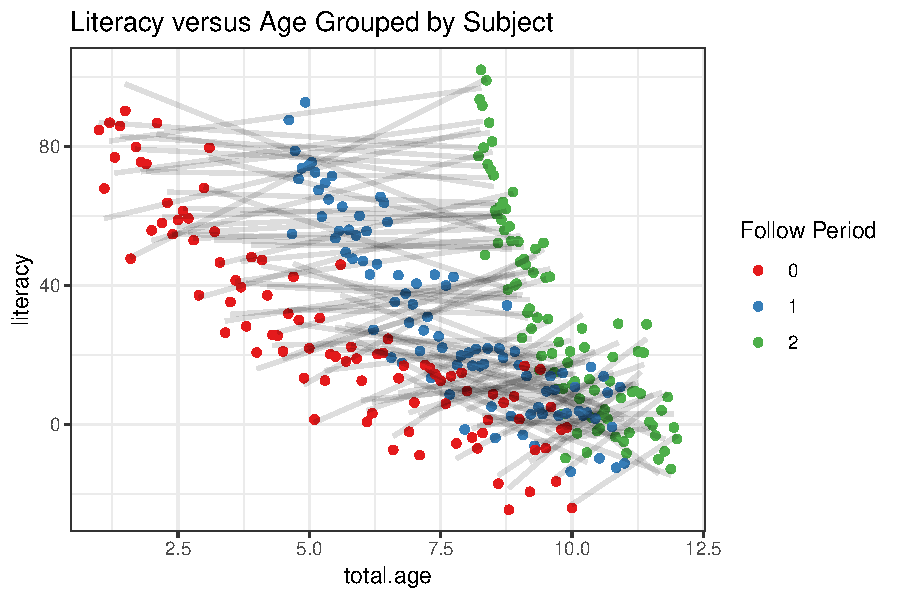
\includegraphics{literacy_versus_age.pdf}
    \caption{Plot of a single realization of the data with $\sigma^2 = 100$. The
      lines are fitted with OLS linear regression conditioned on each subject.}
    \label{fig:literacy_versus_age}
  \end{figure}

  \begin{description}
  \item[Solution:] A single realization is plotted in Figure
    \ref{fig:literacy_versus_age}. By looking at the data from follow period $0$
    and comparing subjects, one can identify the marginal trend: literacy
    decreases with the base age, so younger subjects generally have higher
    literacy. To see the conditional trend, one looks within each subject:
    generally, as a subject ages, their literacy increases. This conditional
    trend isn't very strong, however, since the variance is rather large
    relative to the effect size.
  \end{description}
  
\end{enumerate}
{\em Based on the plot you have generated (and experience from homework 1), it should be clear that
trying to estimate $\beta_L$ by fitting a partitioned model in which you treat $f(x)$ as linear will not work.  
You explain this to your collaborator and propose to fit a model where you include a fixed effect to stratify by
subject.  Your collaborator is sympathetic to the need to deal with confounding but is concerned that fitting a model with $92$ parameters and only $91 \times 3=273$ observations is not a very good idea.  He suggests,
as an alternative, adjusting for subject using a random intercept in a linear mixed effects model (fit using REML, of course).}
\begin{enumerate}[(a)]
\addtocounter{enumi}{1}
\item{\em Explain to your collaborator, purely in words, why this is a bad idea.}
  \begin{description}
  \item[Solution:] The random effects model assumes that the subject-specific
    adjustments to the intercept are normally distributed. This is not the
    case. See the histograms in Figure \ref{fig:literacy_by_follow_period}. In
    particular, look at the base literacy rate in follow period 0. This
    distribution is not normal and skews left. Thus, a random effects model
    would not properly account for the subject-specific variation.
  \end{description}
\end{enumerate}

\begin{figure}
  \centering
  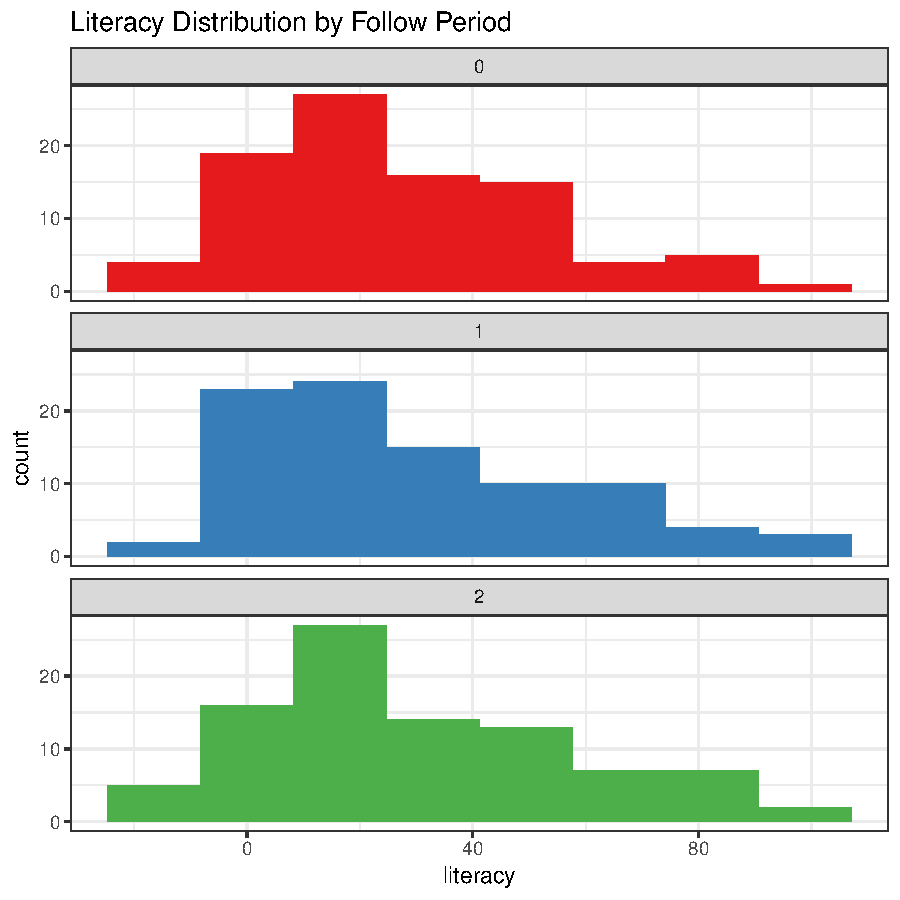
\includegraphics{literacy_by_follow_period.pdf}
  \caption{Distribution of literacy by the follow period. One sees that the
    distribution skews left and is not normal.}
  \label{fig:literacy_by_follow_period}
\end{figure}

{\em Although you're sure that your explanation should have been persuausive, your collaborator is not yet convinced.  So you conduct a simulation to 
further elucidate the differences between estimating $\beta_L$ from models with
fixed effects and random effects for subject-specific intercepts.  }

\begin{enumerate}[(a)]
\addtocounter{enumi}{2}
\item {\em Write down the mathematical form of the two models you will be fitting and describe the simulation study.}

  \begin{description}
  \item[Solution:] Let $Y_i$ be the observed literacy rates for subject $i$. Let
    $X_i$ be the covariates for subject $i$: an $m \times 2$ matrix of $1$s in
    the first column and delta ages in the second. $\beta = \begin{pmatrix}
      \beta_0 & \beta_L
    \end{pmatrix}^\intercal$ are the fixed effect coefficients for the intercept
    and delta age.

    In the random effects model, we have that
    \begin{align}
      Y_i
      &= X_i\beta + \mathbf{1}\gamma_i + \epsilon_i
        \label{eqn:random_effects_model} \\
      \gamma_i
      &\sim \mathcal{N}\left(0, \sigma_\gamma^2\right) \nonumber \\
      \epsilon_{ij}
      &\sim \mathcal{N}\left(0, \sigma^2\right). \nonumber
    \end{align}
    The $\gamma_i$ induces within-subject correlation. This model will be fit
    with a restricted maximum likelihood (REML) procedure.

    In the fixed effects model, we have that
    \begin{align}
      Y_i
      &= \begin{cases}
        X_i\beta + \epsilon_i, & i = 1 \\
        X_i\beta + \mathbf{1}\alpha_i + \epsilon_i, & i \neq 1
      \end{cases} \label{eqn:fixed_effects_model} \\
      \epsilon_{ij}
      &\sim \mathcal{N}\left(0, \sigma^2\right). \nonumber
    \end{align}
    The $\alpha_i$ are subject-specific intercepts and considered fixed effects
    in this case. We can fit this model with ordinary least squares (OLS)
    regression that maximizes likelihood.
  \end{description}


\item {\em  Present and explain the results of your simulation study to your collaborator, highlighting the simulation-based estimates of bias and standard errors of the $\hat{\beta}_L$ you obtain from each model and how these relate to his suggestion.}

  % latex table generated in R 3.5.2 by xtable 1.8-3 package
% Sun Mar  3 17:46:58 2019
\begin{table}[ht]
\centering
\begingroup\small
\begin{tabular}{rrrrrr}
  \toprule
 & $\mathbb{E}\left[\hat{\beta}_L\right]$ & $\mathbb{E}\left[\hat{\sigma}_{\hat{\beta}_L}\right]$ & Sample $\hat{\sigma}_{\hat{\beta}_L}$ & $\mathbb{E}\left[\hat{\sigma}\right]$ & $\mathbb{E}\left[\hat{\sigma}_{\gamma}\right]$ \\ 
  \midrule
Random Effects Intercept & 1.276229 & 0.320826 & 0.328489 & 10.008001 & 24.350760 \\ 
  Fixed Effects Intercept & 0.998420 & 0.321478 & 0.323965 & 9.983993 &  \\ 
   \bottomrule
\end{tabular}
\endgroup
\caption{\small Results of a simulation study comparing modeling the  subject-specific intercepts as a random effect or fixed effect. Parameter estimates were averaged over simulations. Standard errors for $\hat{\beta_L}$ are calculated two ways: (1) assuming the model is correct ($\mathbb{E}\left[\hat{\sigma}_{\hat{\beta}_L}\right]$), and (2) using the $\hat{\beta_L}$ samples (Sample $\hat{\sigma}_{\hat{\beta}_L}$).} 
\label{tab:simulation_comparison}
\end{table}


  \begin{description}
  \item[Solution:] $2^{13}$ simulations were done for each model. Equation
    \ref{eqn:random_effects_model} is used in the random effects intercept
    model, and Equation \ref{eqn:fixed_effects_model} is used in the fixed
    effects intercept model. The results can be seen in Table
    \ref{tab:simulation_comparison}.

    The random effects model has significant bias and overestimates $\beta_L$,
    which has true value $\beta_L = 1$, whereas the fixed effects model appears
    unbiased. The random effects model underestimates the subject-specific
    intercepts and compensates by overestimating $\beta_L$.

    The standard errors of both models agree. The model-based standard errors
    also agree with the simulated standard errors in both models.   
  \end{description}
  

\item {\em  Summarize the estimated values of the residual and random effect variances ($\hat{\sigma}^2$ and $\hat{\sigma}^2_\gamma$, respectively) from your simulations.}

  \begin{description}
  \item[Solution:] $\sigma^2$ measures the variance from the $\epsilon_{ij}$
    term in the model, which is the error in each individual observation. The
    estimated value of the residual variance $\hat{\sigma}^2$ is very accurate
    in both models. See the square root in the
    $\mathbb{E}\left[\hat{\sigma}\right]$ column of
    Table \ref{tab:simulation_comparison}. The actual value is $10$.

    $\sigma^2_L$ measures the variance associated from the $\gamma_i$ term in
    the model, which accounts for subject-level differences. It's only estimated
    in the random effects model by $\hat{\sigma}^2_\gamma$.
  \end{description}
  
\item {\em  Although the subject-specific intercepts in this problem are not really random, there is a natural quantity that you can think of $\hat{\sigma}^2_\gamma$ as trying to estimate.  Calculate this number and call
    it $\sigma_\gamma^2$.  Explain how your estimates $\hat{\sigma}^2_\gamma$ compare to  $\sigma_\gamma^2$.}

  \begin{description}
  \item[Solution:] $\sigma_\gamma^2$ can be thought of as the variance in the
    base literacy score. In this case, the base literacy score for subject $i$
    is $f\left(x_{i1}\right) = f\left(1+0.1(i-1)\right)$.

    We have that the standard error in base literacy is
    \begin{equation}
      \sigma_\gamma = \sqrt{\frac{1}{n}\sum_{i=1}^n\left(
          f\left(x_{i1}\right) - \frac{1}{n}\sum_{j=1}^nf\left(x_{1}\right)
        \right)^2} \approx 24.433055478.
      \label{eqn:sigma_gamma}
    \end{equation}
    Indeed, this number is very close to our estimate in the
    $\mathbb{E}\left[\hat{\sigma}_\gamma\right]$ column of Table
    \ref{tab:simulation_comparison}.
  \end{description}
  
\end{enumerate}

{\em For the remainder of the problem, consider the idealized situation where REML always estimates the variances
exactly, meaning $\sigma^2=\hat{\sigma}^2=100$ and $\sigma^2_\gamma=\hat{\sigma}^2_\gamma$.}
\begin{enumerate}[(a)]
\addtocounter{enumi}{6}
\item {\em Calculate the exact (to your computer's numerical precision) bias of $\hat{\beta}_L$ from the random effect model as an estimator for $\beta_L$.  Report your answer to five significant digits.  Do this calculation two ways, first by interpreting the estimation procedure as GLS regression and then by interpreting it as penalized OLS regression.}

\begin{description}
\item[Solution:] Thre random effects model described in Equation
  \ref{eqn:random_effects_model} estimates $\beta_L$ with a bias of
  $\boxed{0.27288324.}$ The calculations are described below.

  The random effects model implies a subject-specific covariance structure of
  \begin{equation}
    \Sigma_i = \sigma^2_\gamma\mathbf{1}\mathbf{1}^\intercal + \sigma^2I,
    \label{eqn:sigma_i}
  \end{equation}
  where we use Equation \ref{eqn:sigma_gamma} to compute
  $\sigma_\gamma^2$. Using Equation \ref{eqn:sigma_i}, we can compute
  $\hat{\beta}$ with the generalized least squares (GLS) estimator:
  \begin{equation}
    \hat{\beta}_{\text{GLS}} = \left(\sum_{i=1}^nX_i^\intercal \Sigma_i^{-1}X_i\right)^{-1}
    \sum_{i=1}^n X_i^\intercal\Sigma_i^{-1}Y_i.
    \label{eqn:beta_hat_gls}
  \end{equation}
  Equation \ref{eqn:beta_hat_gls} is implemented in
  \texttt{expect.beta.hat.gls}.

  Let $Y$ be the concatenation of the $Y_i$. Let $X$ be the $nm \times (n + 2)$
  design matrix for an overspecified OLS problem. The first two columns are a
  result of stacking the $X_i$ and the last $j + 2$ column represents an
  indicator for subject $j$. The first 2 coefficients are the fixed effects, and
  the remaining $n$ are random effects, which we want to penalize. In penalized
  OLS regression, we are minimizing the mean squared error with an additional
  penalty term:
  \begin{align}
    \hat{\beta}_{\text{OLS}}
    &= \argmin_{\beta}\left[
      \left(Y - X\beta\right)^\intercal\left(Y - X\beta\right)
      +
      \beta^\intercal Q\beta
      \right] \label{eqn:penalized_ols_objective}\\
    \text{where}~
    Q &= \begin{pmatrix}
      0 \cdot I_2 & \mathbf{0} \\
      \mathbf{0} & \frac{\sigma^2}{\sigma_\gamma^2} \cdot I_n
    \end{pmatrix}, \nonumber
  \end{align}
  which means the fixed effects are not penalized, and the random effects are
  penalized with weight $\frac{\sigma^2}{\sigma_\gamma^2}$ as in slide 3.70 of
  the course notes.

  This is just ridge regression and has the closed-formed solution:
  \begin{equation}
    \hat{\beta}_{\text{OLS}}
    = \begin{pmatrix}
      \hat{\beta}_0 \\
      \hat{\beta}_L \\
      \hat{\gamma}_1 \\
      \hat{\gamma}_2 \\
      \vdots \\
      \hat{\gamma}_n
    \end{pmatrix}
    = \left(X^\intercal X + Q\right)^{-1}X^\intercal Y.
    \label{eqn:beta_hat_ols_closed_form}
  \end{equation}
  Equation \ref{eqn:beta_hat_ols_closed_form} is implemented in
  \texttt{expect.beta.hat.ridge}.
  
  Applying Equation \ref{eqn:beta_hat_ols_closed_form} means solving a system of
  equations with $O(n)$ variables, which has complexity $O\left(n^3\right)$. If
  this is too expensive, gradient-based methods applied to Equation
  \ref{eqn:penalized_ols_objective} can be used. The gradient-based method is
  implemented in \texttt{expect.beta.hat.penalized} and relies on the
  \texttt{penalized} package.

  For both Equations \ref{eqn:penalized_ols_objective} and
  \ref{eqn:beta_hat_ols_closed_form}, we can use linearity of expectation to
  calculate the expected value,
  $\mathbb{E}\left[Y_{ij}\right] = f\left(x_{i1}\right) + \beta_Lx_{ij}$.

  With $\sigma^2 = 100$, all three functions produce
  $\mathbb{E}\left[\hat{\beta}_L\right] = 1.27288324$, so there is bias of
  $\boxed{0.27288324}$ in the random effects model. This agrees with the results
  of the simulation study in Table \ref{tab:simulation_comparison}.

  It turns out that the closed form solution to ridge regression in Equation
  \ref{eqn:beta_hat_ols_closed_form} is fastest.
\end{description}

\item  {\em Using the calculation from part (g) of this problem, plot the bias of $\hat{\beta}_L$ as
a function of $\sigma^2$, over an interesting range of choices for $\sigma^2$ (continue to use the same fixed value
of $\sigma^2_\gamma$ you estimated from the data).}

\begin{figure}
  \centering
  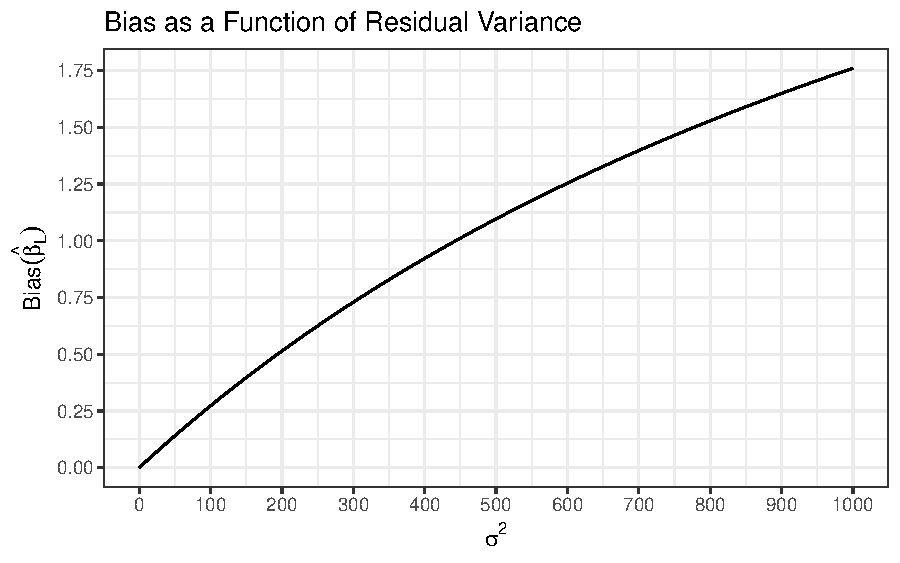
\includegraphics{bias_variance_plot.pdf}
  \caption{The bias of $\hat{\beta}_L$ is calculated with Equation
    \ref{eqn:beta_hat_ols_closed_form} varying $\sigma^2$ from $10^{-1}$ to
    $10^3$.}
  \label{fig:bias_variance}
\end{figure}

\begin{description}
\item[Solution:] See Figure \ref{fig:bias_variance}. The bias increases with
  $\sigma^2$.
\end{description}

\item {\em Explain your plot from part (h) of this problem to your collaborator.  Offer two explanations for the pattern in the plot, one based on the clustered WLS (equivalently, GLS) intepretation and the other based on the penalized OLS interpretation of the linear mixed effects model estimation algorithm.}

  \begin{description}
  \item[Solution:] Recall the model in Equation
    \ref{eqn:random_effects_model}. Consider the random vectors
    $Y_i - X_i\beta = \mathbf{1}\gamma_i + \epsilon_i$ obtained from subtracting
    out the fixed effects. The residuals can be decomposed into a within-subject
    and independent component.

    \begin{description}
    \item[GLS:] From the GLS perspective, the random vector has distribution
      $\mathcal{N}\left(\mathbf{0}, \Sigma_i\right)$, where $\Sigma_i$ takes the
      form in Equation \ref{eqn:sigma_i}, and we're maximizing likelihood.

      Small values of $\sigma^2$ mean that the entries of the random vector are
      highly correlated, so each entry of the random vector should be almost
      identical. In this way, the model is encouraged to find the subject effect
      $f\left(x_{i1}\right)$ of the true model. The model weights the
      $\mathbf{1}\gamma_i$ term appropriately, and the bias of $\hat{\beta}_L$
      is small.

      Large values of $\sigma^2$ mean the entries of the random vector are
      uncorrelated, so there is no need to choose $\hat{\beta}$ such that the
      entries of the random vector are similar. The model is not able to
      disentangle the subject effect $f\left(x_{i1}\right)$ from the noise
      random vector $\epsilon_i$. The difference between a subject's base
      literacy and $\beta_0$ is considered noise. Base literacy skews left (see
      Figure \ref{fig:literacy_by_follow_period}), so $\beta_0$ is
      underestimated. The model compensates by overestimating $\beta_L$. As
      $\sigma^2 \rightarrow \infty$, the model approaches the OLS estimates.
      
    \item[Penalized OLS:] From the penalized OLS perspective, there is no
      within-subject correlation structure. The $\gamma_i$ are just additional
      fixed effects that are encouraged to be close to $0$ by the objective
      function in Equation \ref{eqn:penalized_ols_objective}. $\sigma^2$ is
      proportional to the penalty.

      When the penalty is small, $\gamma_i$ are allowed to vary freely. Since
      the true model will minimize the expected mean squared error,
      $\gamma_i \rightarrow f\left(x_{i1}\right) - \beta_0$ as
      $\sigma^2 \rightarrow 0$. Thus, we estimate $\beta_L$ with small bias.

      When the penalty is large, $\gamma_i$ are pushed towards $0$. As
      $\sigma^2$ gets large, the penalized OLS estimate approaches the estimate
      of OLS with just two coefficients $\beta_0$ and $\beta_L$. Without these
      additional effects, the left skew of base literacy results in
      underestimating $\beta_0$ (see Figure
      \ref{fig:literacy_by_follow_period}). To fit the data better in this
      situation, $\beta_L$ is overestimated.
    \end{description}
  \end{description}
\item {\em Your collaborator is nearly convinced, but not quite.  He reminds you that you
once told him mixed model effect estimates can be thought of as solutions to a GLS problem and that
any old GLS estimator will do (regardless of correlation structure) to consistently estimate the 
coefficients in a linear regression model. Explain why this argument doesn't apply in the present situation.}

\begin{description}
\item[Solution:] Consider the GLS estimator in Equation \ref{eqn:beta_hat_gls}. We have
  \begin{align}
    \mathbb{E}\left[\hat{\beta}_{\text{GLS}}\right]
    &=
    \left(\sum_{i=1}^nX_i^\intercal \Sigma_i^{-1}X_i\right)^{-1}
      \sum_{i=1}^n X_i^\intercal\Sigma_i^{-1}\mathbb{E}\left[Y_i\right] \\
    &= \left(\sum_{i=1}^nX_i^\intercal \Sigma_i^{-1}X_i\right)^{-1}
      \sum_{i=1}^n X_i^\intercal\Sigma_i^{-1}\mathbb{E}\left[X_i\beta + \mathbf{1}\gamma_i + \epsilon_i\right] \nonumber\\
    &= \beta + \left(\sum_{i=1}^nX_i^\intercal \Sigma_i^{-1}X_i\right)^{-1}
      \sum_{i=1}^n X_i^\intercal\Sigma_i^{-1}\mathbf{1}\mathbb{E}\left[\gamma_i\right]. \nonumber
  \end{align}
  The GLS estimator is only unbiased if and only if
  $\left(\sum_{i=1}^nX_i^\intercal \Sigma_i^{-1}X_i\right)^{-1}\sum_{i=1}^n
  X_i^\intercal\Sigma_i^{-1}\mathbf{1}\mathbb{E}\left[\gamma_i\right] =
  \mathbf{0}$.

  In the true model, the $\gamma_i$ are not random. They are fixed
  $\gamma_i = f\left(x_{i1}\right) - \beta_0$, where
  $\beta_0 = \frac{1}{n}\sum_{i=1}^nf\left(x_{i1}\right)$. A realization of the
  $f\left(x_{i1}\right)$ with noise can be seen in Figure
  \ref{fig:literacy_by_follow_period} in the follow period $0$ histogram. The
  distribution skews left and is not normal. Morever, in Figure
  \ref{fig:literacy_versus_age}, one sees that it's value is correlated with
  $x_{i1}$.

  GLS is fitted by maximizing likelihood and assumes normality, so it adjusts
  the estimate of $\hat{\beta}$ so that the distribution of the
  $\hat{\gamma}_{i} = Y_{ij} - \hat{\beta}_0 - \hat{\beta}_{L}x_{ij}$ fits a
  normal distribution with mean $0$. $\gamma_i$ is the source of within-subject
  correlation. In this way, there is a tension between correctly accounting for
  the within-subject correlation and having the residuals $Y_{i} - X_{i}\beta$
  maximize the multivariate normal likelihood model.

  Given that the true distribution is not normal, the fitting procedure must
  choose biased values for $\hat{\beta}$. In particular, the left skew results
  in an underestimate of $\beta_0$. To better fit the data, $\beta_L$ must then
  be overestimated.
\end{description}
\end{enumerate}

\section*{Appendix}

The following pages contain code to reproduce tables and plots. Functions to
computed the expected value of $\hat{\beta}$ are implemented.
\clearpage
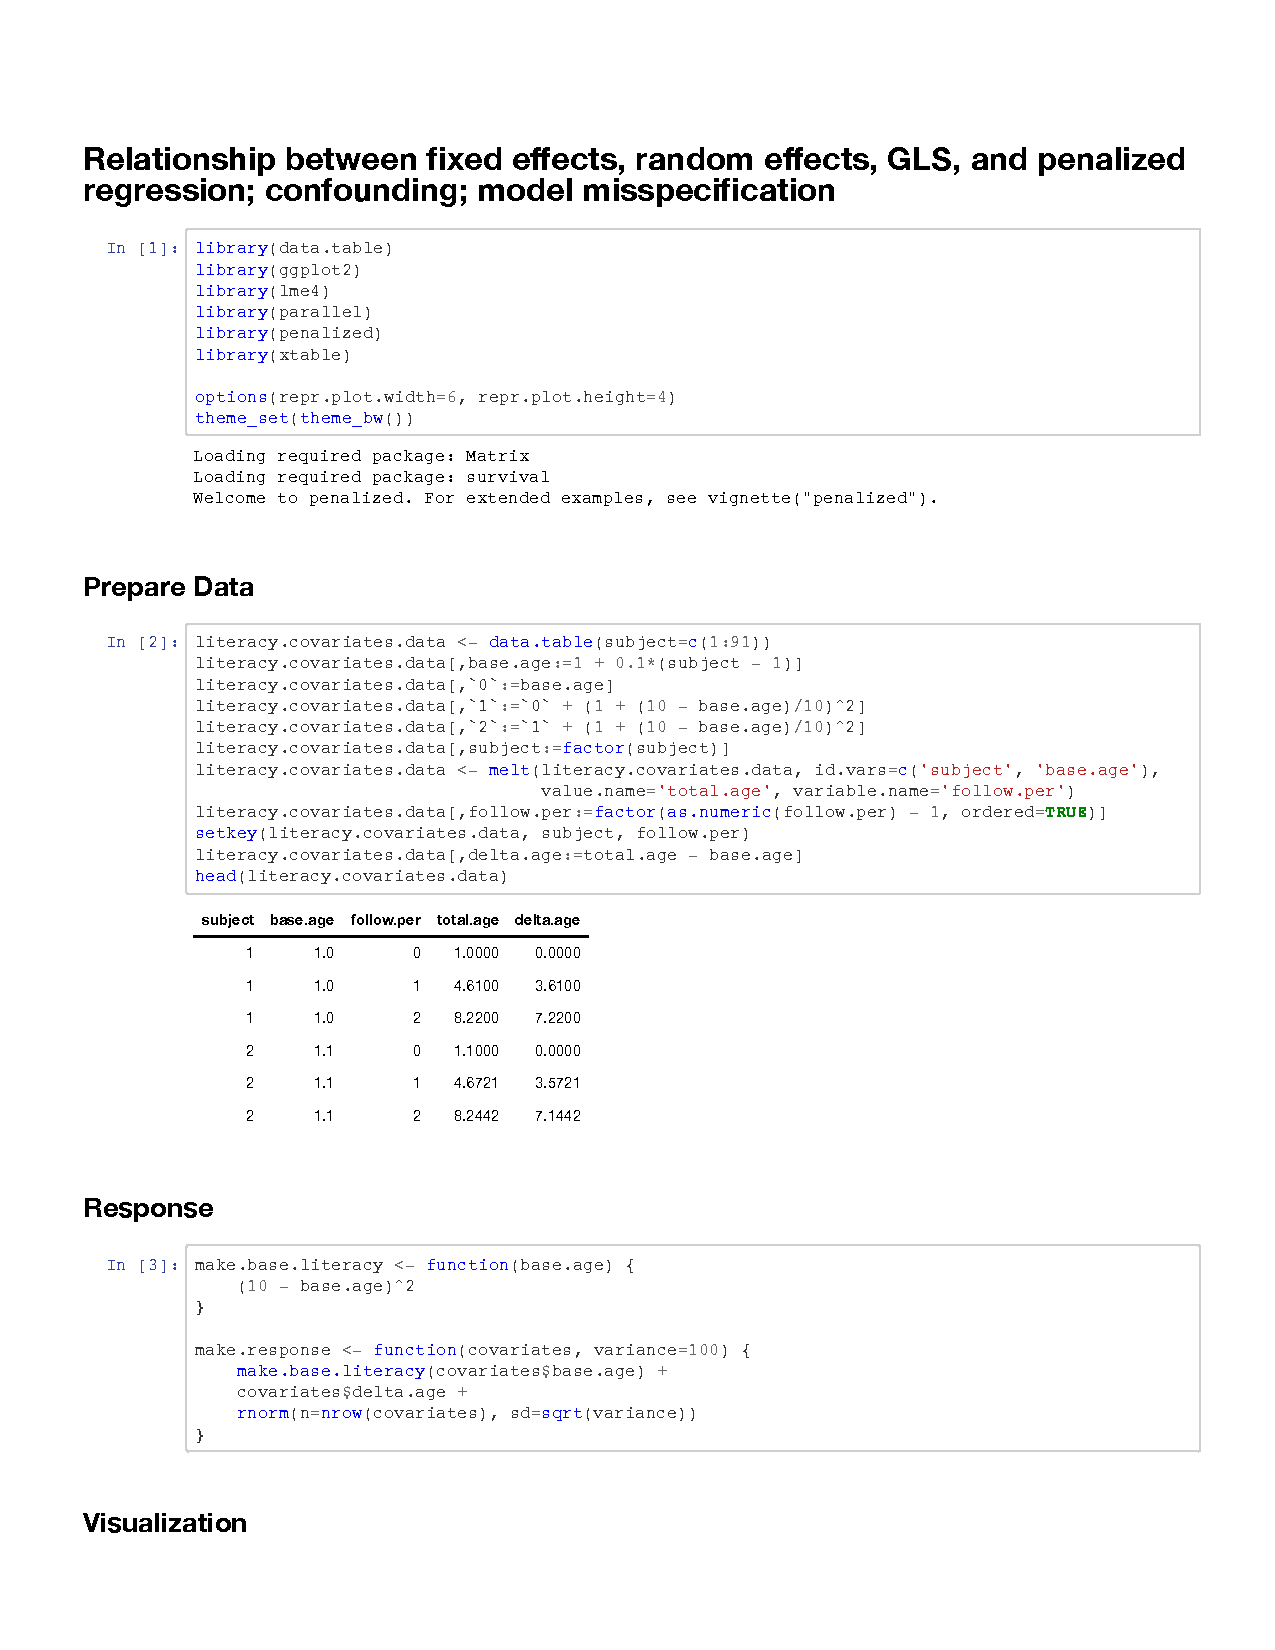
\includepdf[pages=-]{literacy.pdf}

\end{document}